\documentclass[tikz, border=10pt]{standalone}
\usetikzlibrary{positioning, arrows.meta, calc}
\usepackage{luatexja-fontspec}
\setmainjfont{HiraMaruProN-W4} % ヒラギノ丸ゴシックを指定

\begin{document}
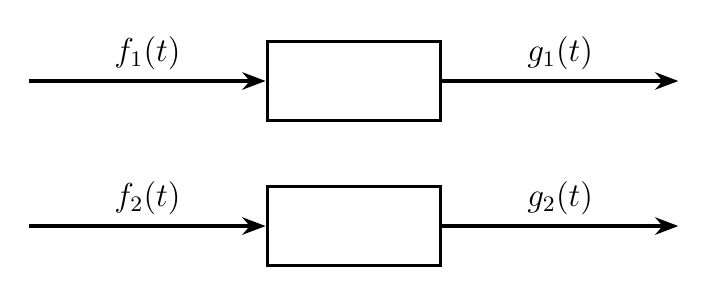
\begin{tikzpicture}[
  very thick,             % 線を太めにする
  >=Stealth,              % 綺麗な矢じりを使用
  font=\large,            % フォントサイズを一括で大きくする
  block/.style={draw, rectangle, minimum width=2.2cm, minimum height=1cm},
  node distance=0.8cm     % 1番と2番の間隔を適切な 0.8cm に固定
  ]

  % --- 1段目 (t_1) ---
  \node [block] (sys1) {};
  \draw [->] (sys1.west) ++(-3.0,0) -- (sys1.west) node[midway, above] {$f_{1}(t)$};
  \draw [->] (sys1.east) -- ++(3.0,0) node[midway, above] {$g_{1}(t)$};

  % --- 2段目 (t_2) ---
  % 1つ目のboxから 0.8cm 下に配置（あきすぎを解消）
  \node [block, below=of sys1] (sys2) {};
  \draw [->] (sys2.west) ++(-3.0,0) -- (sys2.west) node[midway, above] {$f_{2}(t)$};
  \draw [->] (sys2.east) -- ++(3.0,0) node[midway, above] {$g_{2}(t)$};

\end{tikzpicture}
\end{document}


